\documentclass[a4paper,12pt,final]{memoir}

% misc
\renewcommand{\familydefault}{bch}	% font
\pagestyle{empty}					% no pagenumbering
\setlength{\parindent}{0pt}			% no paragraph indentation


% required packages (add your own)
\usepackage{polski}
\usepackage[utf8]{inputenc}
\usepackage{flowfram}										% column layout
\usepackage[top=1cm,left=1cm,right=1cm,bottom=1cm]{geometry}% margins
\usepackage{graphicx}										% figures
\usepackage{url}											% URLs
\usepackage[usenames,dvipsnames]{xcolor}					% color
\usepackage{multicol}										% columns env.
	\setlength{\multicolsep}{0pt}
\usepackage{paralist}										% compact lists
\usepackage{tikz}

%%%%%%%%%%%%%%%%%%%%%%%%%%%%%%%%%%%%%
% Create column layout
%%%%%%%%%%%%%%%%%%%%%%%%%%%%%%%%%%%%%
% define length commands
\setlength{\vcolumnsep}{\baselineskip}
\setlength{\columnsep}{\vcolumnsep}

% left frame
\newflowframe{0.2\textwidth}{\textheight}{0pt}{0pt}[left]
	\newlength{\LeftMainSep}
	\setlength{\LeftMainSep}{0.2\textwidth}
	\addtolength{\LeftMainSep}{1\columnsep}
 
% small static frame for the vertical line
\newstaticframe{1.5pt}{\textheight}{\LeftMainSep}{0pt}
 
% content of the static frame
\begin{staticcontents}{1}
\hfill
\tikz{%
	\draw[loosely dotted,color=ForestGreen,line width=1.5pt,yshift=0]
	(0,0) -- (0,\textheight);}%
\hfill\mbox{}
\end{staticcontents}
 
% right frame
\addtolength{\LeftMainSep}{1.5pt}
\addtolength{\LeftMainSep}{1\columnsep}
\newflowframe{0.7\textwidth}{\textheight}{\LeftMainSep}{0pt}[main01]


%%%%%%%%%%%%%%%%%%%%%%%%%%%%%%%%%%%%%
% define macros (for convience)
%%%%%%%%%%%%%%%%%%%%%%%%%%%%%%%%%%%%%
\newcommand{\Sep}{\vspace{1.5em}}
\newcommand{\SmallSep}{\vspace{0.5em}}

\newenvironment{Career Profile}
	{\ignorespaces\textbf{\color{ForestGreen} Career Profile}}
	{\Sep\ignorespacesafterend}
	
\newenvironment{Key experience}
	{\ignorespaces\textbf{\color{ForestGreen} Key experience}}
	{\Sep\ignorespacesafterend}
\newcommand{\CVSection}[1]
	{\Large\textbf{#1}\par
	\SmallSep\normalsize\normalfont}

\newcommand{\CVItem}[1]
	{\textbf{\color{ForestGreen} #1}}


%%%%%%%%%%%%%%%%%%%%%%%%%%%%%%%%%%%%%
% Begin document
%%%%%%%%%%%%%%%%%%%%%%%%%%%%%%%%%%%%%
\begin{document}

% Left frame
%%%%%%%%%%%%%%%%%%%%
%
% Upload your own photo using the files menu
\begin{figure}
	\hfill
	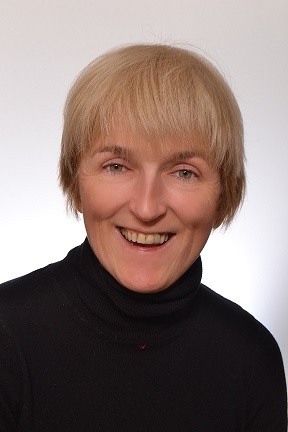
\includegraphics{zeby.JPG}
% * <zuzanna.onderko@gmail.com> 2016-07-02T13:33:03.979Z:
%
% ^.
	\vspace{-7cm}
\end{figure}

\begin{flushright}
	\small
	\color{White}....................................\\
	\Sep
	\color{Black}
	Beata Greń-Onderko \\
	\url{beongren@gmail.com}  \\
	(+44) 7448 245462\\
	d.o.b.: 31st August 1963\\
	Polish full driving license\\
	CRB on demand
\end{flushright}\normalsize
\framebreak


% Right frame
%%%%%%%%%%%%%%%%%%%%
\Huge\bfseries {\color{ForestGreen} Beata Greń-Onderko} \\
\Large\bfseries  Weekend Cook \\

\normalsize\normalfont

% Career Profile
\begin{Career Profile} 
I am a committed, hard working person who wants to make use of her abilites to cook good, healthy and natural food. I was always passionate about how diet influences human health, and I am still up to date with the newest dietary recomendations. 

\end{Career Profile}

%Key experience
\begin{Key experience}
I regularly cook meal for an older lady, and sometimes help with health care. These meals are always made with very fresh ingredients. She particularly likes the soups that I make. I work in Westabank care home as a cook and my duties include cooking for at least 40 residents. 
\begin{itemize}
\item hands-on experience of preparing food for large number of people
\item good understanding of foods and nutrition suited to older people and basic hygiene good practice
\item good knowledge of vegetarian dishes
\item a good team worker
\item a caring attitude to older people
\item reliability and punctuality
\item an awarness of costs in food preparation and interest in cuisine from different countries
\item a willigness to learn and undertake an further training necessary to do a good job.
\item an ability to learn quickly
\end{itemize}
\end{Key experience}

% Work experience
\CVSection{Work experience}

\CVItem{20th October 2016- ...}\\
Weekend Cook in Westbank Care Home \\
\begin{itemize}
\item{Cooking for more than 40 residents}
\item{Preparing breakfast, lunch, dinner, desserts, birthday cakes}
\item{Works alone or with a help of the kitchen assistant}
\item{Approximately 24 hours per week}
\end{itemize}

\CVItem{Summer 2016 - ...}\\
Occasionally working as a cleaner in Bridge House Hotel.
\begin{itemize}
\item{luxury hotel standards}
\item{cleaning 6-8 rooms}
\end{itemize}
\clearpage
\framebreak
\framebreak
\CVItem{17th May 2016 - October 2016}\\
Sales assistant in Euro Garages (Ross-On-Wye) FULL TIME
\SmallSep

\CVItem{ 8th May 2016 - ...}\\
Cleaner (PART TIME) at Parkfields Country House. Duties: keeping all areas of Parkfields Country house clean and tidy, sorting laundry, dusting, polishing, sweeping.
\SmallSep


\CVItem{September 2015-April 2016}\\
Au pair for two children : girl 22 months, girl 4.5 years old in Ross-on-Wye, UK
\SmallSep

%Training and Courses 
\CVSection{Training and Courses}
\CVItem{ 03rd October 1985 -19th May 1986}\\
\underline{First aid course} at Polish Red Cross at PRC Wrocław
\SmallSep

\CVItem{August 1986}\\
One month \underline{language scholarship} founded by French Embassy at University of Grenoble, France
\SmallSep

\CVItem{02nd March 2009-30th June 2009	}\\
Training in Social Integration Center (Centrum Integracji Społecznej) in 	Wrocław. Aim: schooling in \underline{licensing and running social cooperative (446 hours)}
\SmallSep

\CVItem{10th September 2009-19th December 2009}\\
\underline{English language course} at Pre-Intermediate level in Yellow Language Center 	Sp. z.o.o  (64 hours)
\SmallSep

\CVItem{January -August 2010 }\\
Participation in „Women professionally active- It's me” project concerning: 60h of \underline{UE projects management} training, 8h of \underline{labour legislation} training, 30h of \underline{computer skills} training (MS Office), 8h of \underline{labour market} training, 8h of \underline{psychology} workshop, 8h \underline{auto presentation} skills training,  \underline{english language course} finished with TOEIC exam
\SmallSep

\CVItem{2009-2011}\\
\underline{French language course} at level B2/C1 in Alliance Francais Language School in Wrocław (3 semesters)
\SmallSep

\CVItem{October 2014-July 2015}\\
\underline{English language course} at A2 level (coursebook A2/B1)
with final exam
\SmallSep

% Education
\CVSection{Education}
\CVItem{1982-1987}\\
Studies at Faculty of National Economics at Oskar Lange's Academy of Economics (now University of Economics) in Wrocław
\SmallSep


% Skills
\CVSection{Skills and Interests}
\CVItem{Languages}
\begin{multicols}{3}
\begin{compactitem}[\color{ForestGreen}$\circ$]
	\item English A2
	\item French  B2
	\item German  A1
\end{compactitem}
\end{multicols}
\SmallSep

\CVItem{Interests}
\begin{multicols}{3}
\begin{compactitem}[\color{ForestGreen}$\circ$]
	\item Natural medicine and herbalism
	\item Gardening
	\item Sports: fitness and skiing 
	\item Classical music 
	\item Films and  festivals
\end{compactitem}
\end{multicols}
\Sep 



%%%%%%%%%%%%%%%%%%%%%%%%%%%%%%%%%%%%%
% End document
%%%%%%%%%%%%%%%%%%%%%%%%%%%%%%%%%%%%%
\end{document}